\documentclass[a4j, 10pt, twocolumn]{ujarticle}
\usepackage[dvipdfmx]{graphicx}
\usepackage[utf8]{inputenc}
\usepackage{url}
\usepackage{sty/abstract}

\def\thline{\noalign{\hrule height 1pt}}
\begin{document}

\title{OCR とラベリングによる書類整理自動化システムの構築と有用性の評価}{}

\year{2025}{1}{23}

\AuthorA{
  \author{嘉松 一汰}
  \belong{15820094}
  \class{}
  \presen{}
}

\Email{}

\Keyword{}
\MKTITLE{}

\renewcommand{\baselinestretch}{1.0}
\setlength{\baselineskip}{1.5zh}
\renewcommand{\textfraction}{0.1}
\renewcommand{\floatsep}{1pt}
\renewcommand{\intextsep}{4pt}
\renewcommand{\textfloatsep}{4pt}

\vspace{-20mm}

\section{はじめに}
\subsection{研究背景}

日本企業の RPA (Robotics Process Automation)導入率は全体で38\%,小企業では25\%となっており,常に少ないことがわかる図~\ref{fig:rpa_rate}.
また,企業と中小企業の間に20\%以上の差があり,術や規模による格差も見て取れる. これらの原因は主に2つある.
1つ目は,RPA は紙媒体の処理等の,ナログの世界で行われる処理は非専門領域であるということである.
具体的には,書き文字横書き文字が混在していたり,字体や特殊文字等の組み合わせも考えられるため,外的な処理までを自動で行う必要があるためである.
2つ目の原因は,媒体の業務を行っているコミュニティの IT 知識の乏しさにある.詳しくは次のセクションで説明する.

\begin{figure}[htbp]
  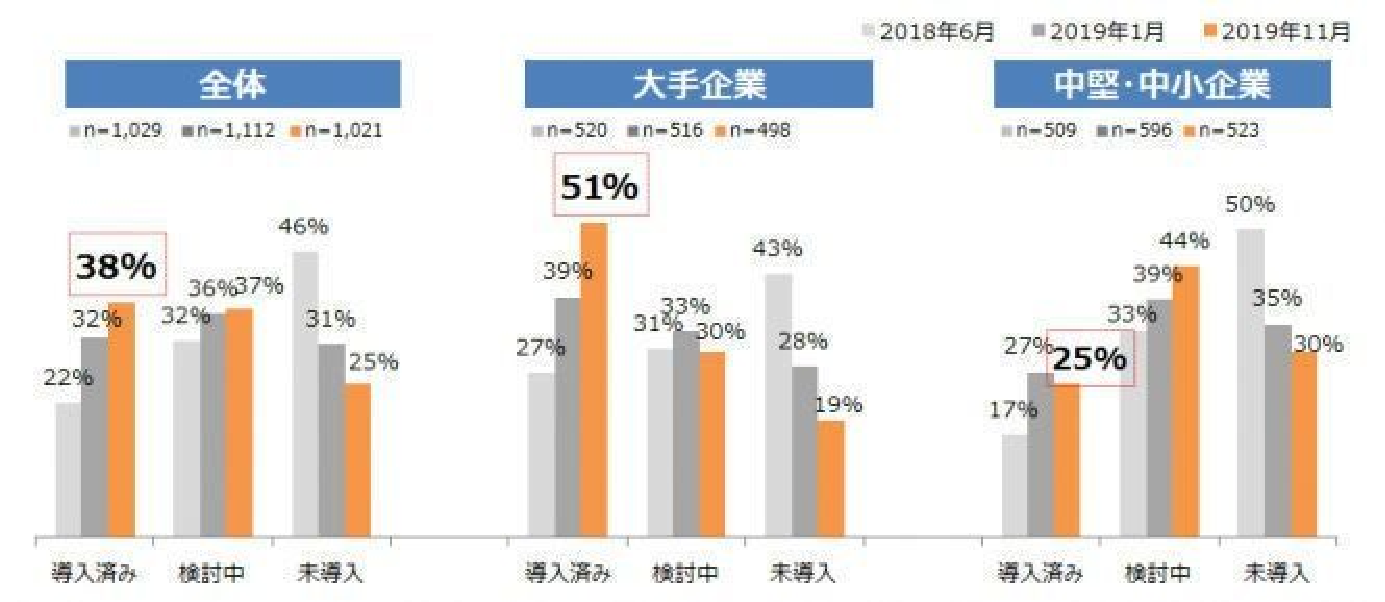
\includegraphics[scale = 0.3]{img/rpa_rate.pdf}
  \caption{企業のRPA導入率}
  \label{fig:rpa_rate}
\end{figure}

\subsection{研究目的}

本研究の目的は,RPA を使用して紙媒体の処理を自動で行うシステムを作成することである.
前述したように,ステム障害への恐怖感や,T知識の乏しさ等によって,IT 知識に乏しいコミュニティが現代には数多く存在します.
このような現状を改善するために,連の流れをRPAにすることで,T知識の有無に関わらず,ステムが運用可能になることを目指す.

\section{関連研究}

本研究では,くまでカテゴライズという目的でシステムを構築しているため,ラスタリング手法とは少し異なる点があるが,ルゴリズム等の観点で参考にしたため,連研究として以下に示す.

\subsection{クラスタリングの既存手法}
\paragraph{非階層的クラスタリング}

目的のデータを事前に定義されたクラスタ数に分解することによって行われるクラスタリング方式のことである.
代表的な手法として,ラスタ内の分散を最小化するようにデータポイントをグループ化するk-meansアルゴリズムが挙げられる.

\paragraph{階層的クラスタリング}

データポイントを機構造の階層に分割して行うクラスタリング方式のことである.代表的な手法には大きく分けて,集型と分割型の2種類がある.
凝集型は,構造の下から上へクラスタを統合していく方法である.対して分割型は,から下へクラスタを分割していく方法である.

\section{提案手法}
\subsection{データベース設計}

本研究で使用するテーブルには3種類あり,~\ref{fig:er_diagram}にこれらのER図を示す

\begin{figure}[htbp]
  \centering
  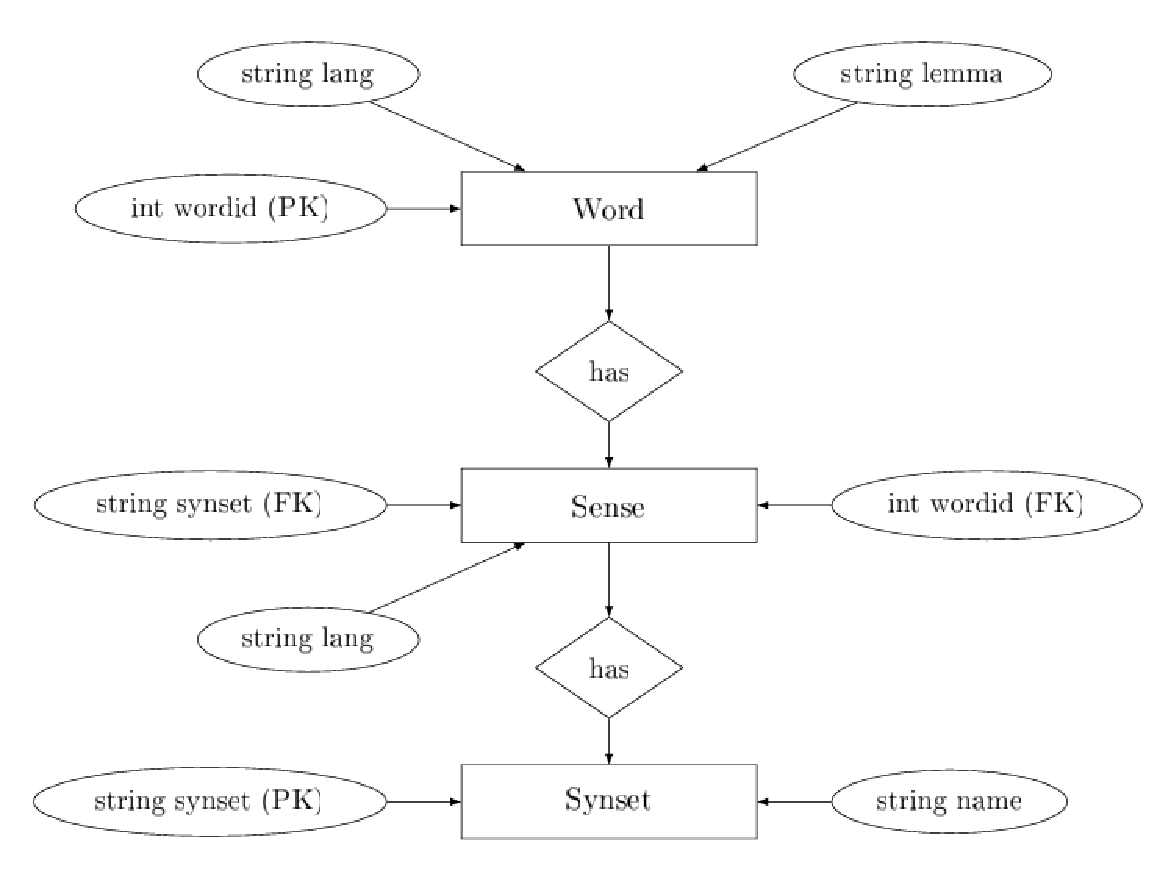
\includegraphics[scale = 0.4]{img/er_diagram.pdf}
  \caption{データベース構成}
  \label{fig:er_diagram}
\end{figure}

\subsection{モデル設計}

\paragraph{Word モデル}
一対多の関係で,数のSense モデルへのリレーションを持っており,Sense モデルを経由して,Synset モデルへのリレーションを辿ることで,語からその定義を取得する.
場合に応じて適切な言語のレコードを活用するため,語での絞り込みを行うスコープを持つ.

\paragraph{Synset モデル}
一対多の関係で,数のWordモデルへのリレーションを持っており,Sense モデルを経由して,Word モデルへのリレーションを辿ることで,定の定義をもつ単語を取得する.
Wordモデルと同様に,語での絞り込みを行うスコープを持つ.

\paragraph{Sense モデル}
上記の2つのモデルそれぞれと一対多のリレーションを持っており,つのモデルの中間テーブルの役割を担う.単語から定義を取得する処理は,ynset テーブルを経由して行う.

\subsection{提案する手法・アプローチ}

カテゴライズしたいドキュメントファイルに対して Google Vision API を使用した OCR を行い,容の単語群を取得する.
その後,ornNetデータベースと連携し,語ごとの定義を取得する.各々の定義を元に単語がどのカテゴリに属するかを判別し,語ごとにラベリングを行う.
ラベリング結果から,終的なドキュメントのカテゴリを決定する.

\section{実験・評価}

本研究の実験で用意するカテゴリは,理,事,務の3種類であり,カテゴリごとに5種類ずつの計15種類のドキュメントに対してカテゴライズ処理を実行し,度の分析を行った.
結果として,理制度にはタイトルごとにばらつきが見られた.特に,字体を含む文書では処理が失敗する傾向が確認された.
一方で,書きや横書きが混在する文書,語表記が一部含まれる文書,シック体や太文字を用いた文書などにおいては,題なく処理が成功している.これらの結果から,ォーマットや字体の違いがOCRの精度に与える影響が明確になった.
また,テゴリごとの処理精度について,理カテゴリにおける精度が他のカテゴリと比べて著しく低いことが確認された.この主な要因としては,理カテゴリの文書に旧字体や特殊な専門用語が多く含まれている点が挙げられる.
これにより,OCR 処理のカテゴリごとの安定性について一定の評価を下すことができる.

\section{考察}
\subsection{結果の解釈}

本システムの優位点については,キュメントの形式に関わらず同様の処理結果を得ることができる点である.文書には,書きや横書き及びそれらの複合など,容の形式はジャンルによって多岐にわたる.
それら全てに対応出来なければ,システムの優位性は著しく低下してしまう.しかし,まざまな形式の文書を実験では用意したが,に形式の差による精度の変化は見受けられなかった.
そのため,システムにおいては,書をアップロードする前に形式を確認する等の校閲を行う必要がなく,の点ではストレスなくシステムを運用することができると考えられる.
本システムの有用性については,~\ref{ch:intro}章で大まかに述べたが,媒体中心の業務に不便を感じている人が現代に多くいるため,のような状況を改善するという観点では,件を満たすことができているといえるだろう.

\subsection{改善点}

本システムの改善点は,字体など,在使用されていない字体を用いた文書に関しては,度が落ちてしまう点である.
具体的には,OCR 処理では不自由なく単語ごとに分けることができているが,ordNet データベースにその単語が存在しないため,語のカテゴリが判別できないことが原因として挙げられる.
改善するためには,状使用しているWordNetデータべースの他に,字字体規範史データセットのような旧字体を扱っているデータベースを使用し,別可能な語彙を拡張することが必要である.
また,状のシステムでは,本語と英語を主な対象としているが,ローバル化が進む現代社会では,言語対応が求められる場面が増えている.
これを実現するためには,言語に特化した語彙データベースを統合し,言語間でのカテゴリ解析を可能にするアルゴリズムの開発が必要である.

\section{おわりに}
\subsection{今後の展望}

今後の展望として,ーザーインターフェース(UI)の最適化も重要である.現状ではシステムのコア機能に重点を置いているが,作の直感性やユーザーエクスペリエンスの向上が求められる.
例えば,析結果を可視化するダッシュボードや,ィードバック機能を備えたインターフェースを実装することで,用者の利便性を高めることが可能である.また,システムをクラウドベースで提供することにより,数のユーザーが同時に利用できる環境を構築し,ケーラビリティを確保することができる.
また,PIを公開することで,のアプリケーションやサービスとの統合を可能にし,ステムの拡張性をさらい高めることも有効である.

\subsection{研究のまとめ}

本システムは,在の業務フローにおける課題を解決し得る有効なツールであると結論付けられる.現代では,後もIT分野の著しい成長に遅れをとったコミュニティを中心に,まざまな業務的ニーズが発生すると考えられる.
本研究では紙媒体中心業務をさらに細分化した,キュメントのカテゴライズ分野に着目してシステムの作成を行ったが,システムのようなソリューションが生み出されることで,IT社会の課題が解決されることを願っている.

\bibliographystyle{junsrt}
\bibliography{biblio}

\end{document}
